\subsection{Experimentación}

En esta sección nos encargaremos de analizar la eficiencia del algoritmo de forma empírica y ver si mantiene alguna relación con la complejidad teórica calculada. Además, analizaremos el comportamiento de las podas en términos de eficiencia.

En cuanto al primer punto, decidimos analizar cuál era el comportamiento del algoritmo en cuánto al tamaño de la entrada. Para ello, optamos por tomar configuraciones iniciales de $1*n$ en donde $n=1,2,...,9$ y observar para cada caso cuántos ciclos insumía el algoritmo en resolverlos. Tomamos la decisión de solo ir hasta $n=9$ por el simple hecho de que se trata de un algoritmo con complejidad exponencial lo cual no permite analizar casos grandes en un tiempo considerable. Los resultados obtenidos fueron los siguientes:

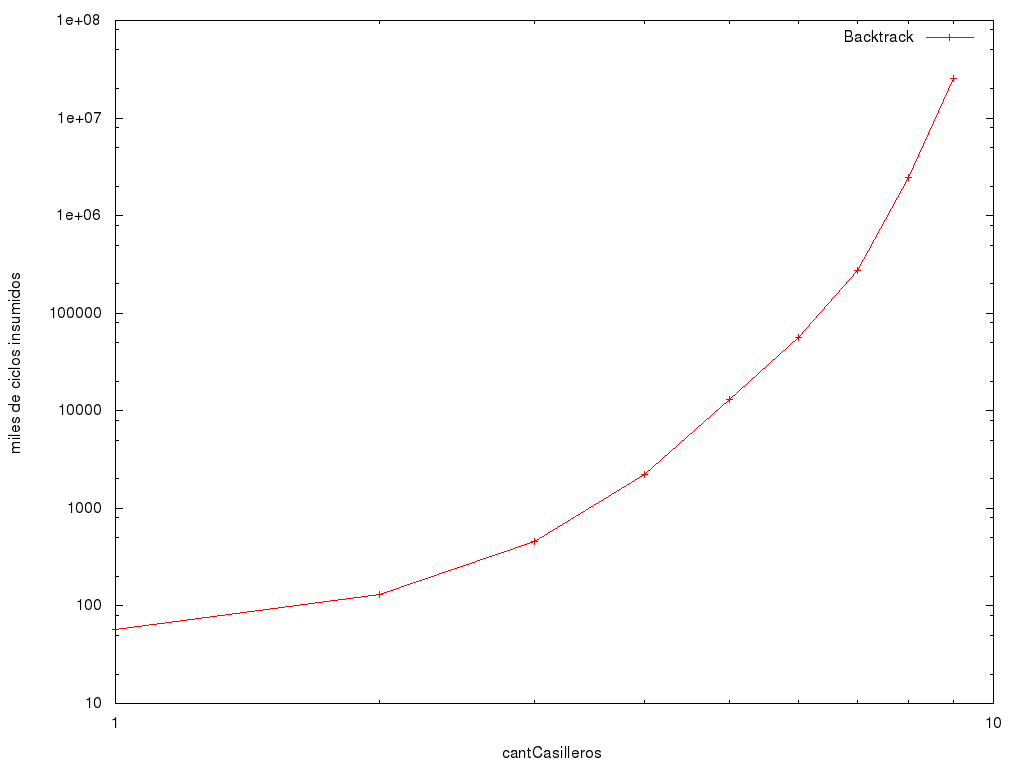
\includegraphics[scale=0.3]{ej3/imgs/ej3-1.png}

Seteamos una escala logarítmica en el gráfico ya que el orden de magnitud de los ciclos insumidos aumentaba de manera considerable lo que no permitía apreciar los resultados. Puede observarse que a medida que incrementamos la cantidad de casilleros simples, el número de ciclos insumidos por el Backtrack crece abruptamente lo cual es lógico ya que la complejidad es exponencial.

Observemos, ahora, cómo se comportan las podas. Analicemos una por una. Veamos el siguiente caso:

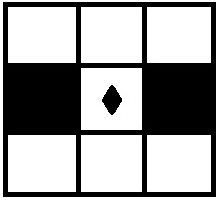
\includegraphics[scale=0.5]{ej3/imgs/ejSinSolucion.png}

La poda $cumpleHastaElMomento$ que se encargaba de verificar que los casilleros importantes fueran cubiertos debería ayudar al algoritmo a devovlver rápidamente que no se encuentra solución. Esto se debe a qué antes de continuar por una rama la poda detecta que no es posible cubrir al casillero imporante con dos sensores. Veamos cómo se comporta el algoritmo con y sin la poda:

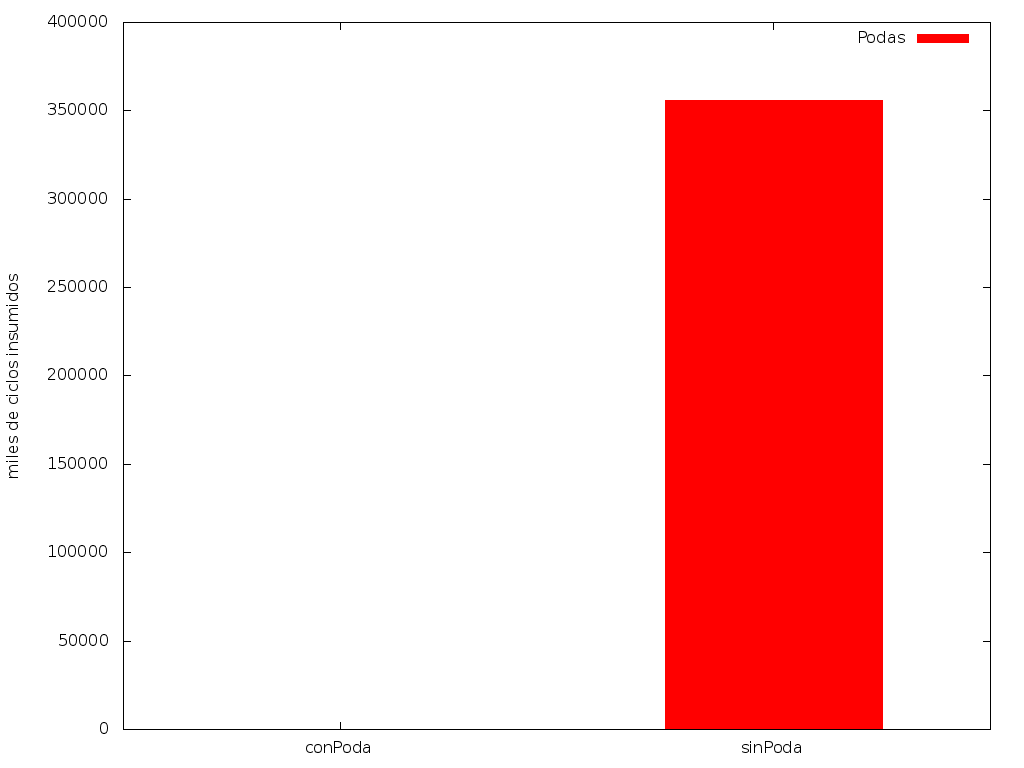
\includegraphics[scale=0.3]{ej3/imgs/cumpleHastaElMomento.png}

La diferencia es tan grande que no llega a verse una barra asociada al algorimo con poda. Veamos cómo funciona la poda $marcarCasilleros$ que se asegura de marcar los casilleros que se encuentran apuntados al momento de insertar un sensor en la grilla. Esta vez probemos la poda en una matriz de $2*2$ llena de casillerosSimples:

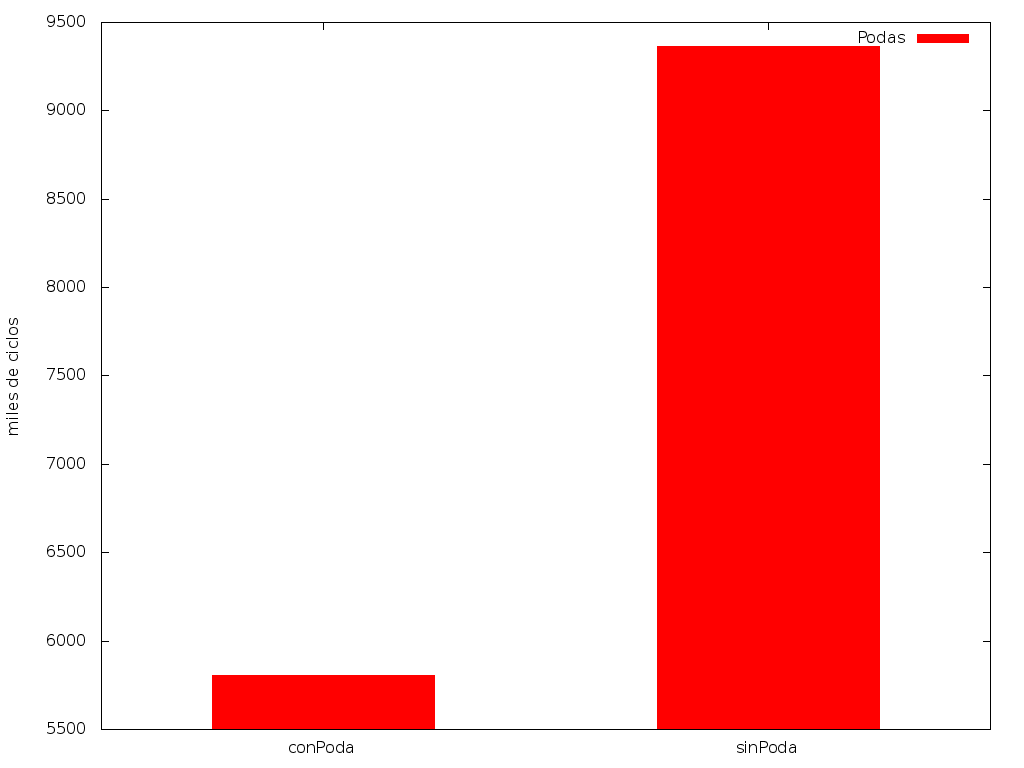
\includegraphics[scale=0.3]{ej3/imgs/22casos.png}

Si bien la diferencia no es tan grande como en el caso anterior podemos apreciar una mejoría importante al utilizar la poda.

Por último, veamos cómo se comportan las podas para el siguiente caso:

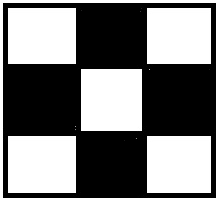
\includegraphics[scale=0.5]{ej3/imgs/ajedrezDibujo.png}

Por lo visto en la sección de complejidad es de esperar que en este ejemplo y en todas las familias de casos similares, las podas no tegan un efecto positivo en cuando a rendimiento. Veamos si es verdad:

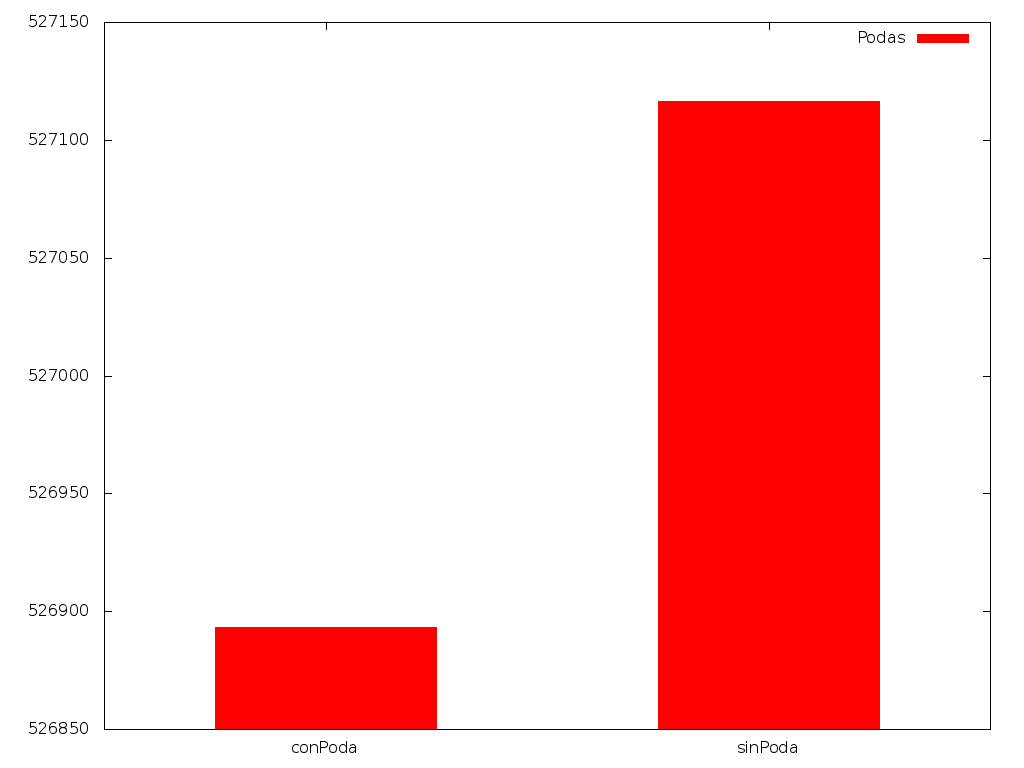
\includegraphics[scale=0.3]{ej3/imgs/ajedrez.png}

Si bien las barras parecen ser muy distintas es importante notar que la diferencia no es tan grande. Mientras uno hace 526000 miles de ciclos, el otro realiza 527000 miles de ciclos.
